% Tento soubor nahraďte vlastním souborem s obsahem práce.
%=========================================================================
% Autoři: Michal Bidlo, Bohuslav Křena, Jaroslav Dytrych, Petr Veigend a Adam Herout 2019
\chapter{Úvod}
TODO

\chapter{Blockchain}\label{chap:blockchain}

Táto kapitola vysvetľuje základné koncepty a pojmy spojené z technológiou blockchain, ako aj samotnú dátovú štruktúru blockchain. Sekcia~\ref{sec:ladger} vysvetľuje pojmi distribuovaná účtovná kniha a blockchain. Ďalej rozoberá vlastnosti a využitie blockchainu. Sekcia~\ref{sec:crypto} vysvetľuje kryptografiu používanú v blockchaine (hashovanie, a asymetrická kryptografia).  Sekcia~\ref{sec:p2p} popisuje peer-to-peer siete a ich využitie v blockchaine. Nazáver sú v sekcii~\ref{sec:data-struct-blockchain} spojené všetky vysvetlené koncepty dokopy a je popísaná samotná dátová štruktúra blockchain.

\section{Distribuovaná účtovná kniha}\label{sec:ladger}
\textit{Účtovná kniha} (anglicky \textit{ledger}) sa v histórii ľudstva dlhodobo používa na záznam rôznych položiek, najčastejšie peňazí a majetku. Príchod digitalizácie a globalizácie presunul tento známy koncept z papierovej podoby do elektronickej. Toto prináša nové výzvy z hľadiska bezpečnosti.
\textit{Distribuovaná účtovná kniha} (anglicky \textit{distributed ledger}) je všeobecne technológia, ktorá poskytuje dôveryhodnú a bezpečnú databázu zdieľanú naprieč viacerými inštitúciami, krajinami a to typicky verejne. Najtypickejším odvetvím využitia distribuovanej účtovnej knihy je bankovníctvo. Banka poskytuje centralizovanú autoritu, ktorá zabezpečuje bezpečnú manipuláciu s peniazmi klientov. Tento koncept označujeme ako centralizovaná účtovná kniha.~\cite{dltUkReport}

V roku 2008 bola publikovaná práca~\cite{satoshiBitcoin}, ktorá navrhla \textit{decentralizovanú} distribuovanú účtovnú knihu. Práca navrhla koncept elektronického platobného systému, ktorého bezpečnosť je založená na kryptografickom dôkaze namiesto dôvere v centralizovanú autoritu. Takáto distribuovaná účtovná kniha sa nazýva \textbf{blockchain}.
\subsection{Vlastnosti blockchainu}
Blockchain je dátová štruktúra, ktorá má nasledujúce vlastnosti:
\begin{itemize}
	\item \textbf{Decentralizácia}: Blockchain funguje nad peer-to-peer sieťou, ktorá nepotrebuje centralizovanú dôveryhodnú autoritu.
	\item \textbf{Auditovateľnosť}: Blockchain v sebe nesie celú histórie zmien jeho obsahu a teda každú zmena stavu dát uložených v blockchaine je možné sledovať.
	\item \textbf{Nemennosť}: Pri správnom použití a dostatočne veľkej sieti nie je možné zmeniť histórie alebo dátový obsah blockchainu.
	\item \textbf{Anonymita}: Užívatelia pracujúci s blockchainom používajú na identifikáciu asymetrickú kryptografiu s digitálnym podpisom. Takýto kryptografický identifikátor neodhaľuje skutočnú identitu užívateľa a pritom umožňuje nepopierateľne určiť vlastníka elektronického zdroja.
\end{itemize}

Tieto vlastnosti blockchainu sú zabezpečené pomocou peer-to-peer siete na ktorej je blockchain postavený (viď sekcia~\ref{sec:p2p}) a taktiež pomocou samotnej dátovej štruktúry, ktorá využíva modernú kryptografiu (viď sekcia~\ref{sec:data-struct-blockchain}).~\cite{horizenAcademy}

\subsection{Aplikačné využitie}

Blockchain bol navrhnutý a po prvýkrát implementovaný za účelom poskytnúť elektronickú peňažnú menu nezávislú od centralizovaného bankovníctva. Tento prvý, a najznámejší, blockchain je Bitcoin~\cite{satoshiBitcoin}. Avšak vlastnosti blockchainovej technológie nachádzajú uplatnenie vo veľkom množstve odvetví. Nasledujúci zoznam vymenúva niekoľko aplikácií, ktoré blockchain môže riešiť~\cite{homoliakBlockchain}:

\begin{itemize}
	\item \textbf{Elektronická peňaženka}: Elektronické peňaženky pre obchod s nejakou formou peňazí (typicky v podobe tokenov). Takéto tokeny sú typicky vlastnené pomocou privátneho kľúča, ktorý má uschovaný majiteľ. Majiteľ môže vlastníctvo tokenov presúvať na iné subjekty v danej sieti.
	\item \textbf{Zmenárne}: V dnešnej dobe existuje veľké množstvo elektoronických peňažných mien postavených nad blockchainom. Takéto meny všeobecne označujeme ako kryptomeny. Z dôvodu veľkého množstva kryptomien sa prirodzene zvyšuje dopyt po zmenárni medzi jednotlivými kryptomenami. Klasická zmenáreň je riešená tradične centralizovanou autoritou. Avšak blockchain je vhodnou technológie aj pre decentralizovanú zmenáreň.
	\item \textbf{Súborové systémy}: V dnešnej dobe už existujú decentralizované súborové systémy založené na peer-to-peer sieťach. Implementácia takéhoto decentralizovaného súborového systému ako blockchain by nám umožnila nepopierateľne a trasovateľne verzovať zmeny v obsahu.
	\item \textbf{Správa identít}: Správa identít je typicky centrálna autorita, ktorá prideľuje pre konkrétne entity určité zdroje na ktoré majú právo. Ide o schému podobnú banke. Blockchain by v tomto prípade opäť umožnil náhradu tejto centralizovanej autority za decentralizovanú sieť.
	\item \textbf{Voľby}: Elektronické voľby sú ďalším vhodným príkladom, kde sa dá efektívne využiť blockchain. Voliace entity predstavujú decentralizovanú sieť a vlastnosti blockchainu zase poskytujú transparentnosť a verejnú overiteľnosť.
	\item \textbf{Reputačné systémy}: Reputačné systémy slúžia na meranie úrovne dôvery v určité entity. Typickým príkladom je reputácia rôznych predajcov na základe hlasovania zákazníkov. Transparentnosť a nemennosť blockchainovej histórie by znížila možnosť manipulácie s reputáciu v prospech nejakej entity.
	\item \textbf{Aukcie}: Elektronická aukcia je služba veľmi podobná elektronickej peňaženke alebo zmenárni s podobnými bezpečnostnými požiadavkami. Tieto vlastnosti by opäť dokázala pokryť technológia blockchain.
\end{itemize}

\section{Kryptografia v blockchaine}\label{sec:crypto}
Pre pochopenie technológie blockchain je potrebná základná znalosť modernej kryptografie. V tejto sekcii je popísaný kryptografická hashovacia funkcia (pozri~\ref{subsec:hash}) a jej využitie na tvorbu dátových štruktúr zabezpečených proti modifikácii obsahu (viď sekcia~\ref{subsec:hash-pointer}). Ďalej je vysvetlený koncept asymetrickej kryptografie a digitálneho podpisu (viď sekcia~\ref{subsec:sign}). Tieto kryptografické primitíva sú základom na ktorom stojí nemennosť, auditovateľnosť a anonymita blockchainu.

\subsection{Hashovacia funkcia}\label{subsec:hash}
Hashovacia funkcia je taká funkcia $h$, ktorá má ako parameter $x$ reťazec bitov ľubovolnej dĺžky a vracia reťazec $y$ s konštantnou dĺžkou(viď rovnica~\ref{eq:hash}). Reťazec $y$ voláme hash. Hashovacia funkcia vracia pre konkrétny vstup vždy rovnaký hash.

\begin{equation} \label{eq:hash}
	h(x) = y
\end{equation}
Kryptografická hashovacia funkcia, alebo tiež jednocestná funkcia (anglicky \textit{one way function}), je taká hashovacia funkcia pre ktorú platia nasledujíce tri vlastnosti:
\begin{enumerate}
	\item Pre daný hash $x$ je výpočetne nezvládnuteľné nájsť správu takú, že $ h(x) = y $. Anglicky voláme túto vlastnosť \textit{first preimage resistant}.
	\item Pre danú správu je výpočetne nezvládnuteľné nájsť inú správu s rovnakým hashom. Anglicky voláme túto vlastnosť \textit{second preimage resistant}.
	\item Pre ľubovoľnú správu je výpočetne nezvládnuteľné nájsť inú správu s rovnakým hashom. Anglicky voláme túto vlastnosť \textit{collision resistant}.
\end{enumerate}

Hashovacie funkcie majú v oblasti počítačovej bezpečnosti dôležité využitie:
\begin{itemize}
	\item Bezpečné ukladanie hesiel: Digitálna služba neukladá v databáze heslo, ale len jeho hash. Pri ukradnutí databázy nedochádza k odhalenie hesiel užívateľov.
	\item Integrita dát: Hashovacia funkcia môže byť použitá na ochranu integrity ľubovoľných dát. Ak spočítate hash veľkého súboru a bezpečne ho uložíte tak ste schopný detekovať, že niekto tento súbor zmenil.
	\item Digitálny podpis: Hashovacia funkcia je kryptografické primitívum potrebné pre vytvorenie digitálneho podpisu.
\end{itemize}
Existuje množstvo hashovacích funkcií. Medzi veľmi známe a používané patrí napríklad MD5 (128 bitový výstup), SHA256 (256 bitový výstup), SHA512 (512 bitový výstup).~\cite{cryptoHandbook, nigelSmartCrypto}

\subsection{Hash ukazovateľ}\label{subsec:hash-pointer}
Hash ukazovateľ (anglicky \textit{hash pointer}) je primitívom pre tvorbu dátových štruktúr s kryptografickým zabezpečením proti manipulácia s obsahom (anglicky \textit{tamper-evident}). Hash ukazovateľ funguje ako klasický ukazovateľ v zozname či strome. Navyše však neumožňuje meniť už pridané prvky. Jediná povolená operácia je pridanie ďalšieho prvku do dátovej štruktúry. 

Obrázok~\ref{img:hash-pointer} demonštruje rozdiel medzi zoznamom vytvoreným pomocou klasických ukazovateľov a pomocou hash ukazovateľov. Bežný zoznam umožňuje pozmeniť ľubovoľný už existujúci prvok nezávisle na zvyšku zoznamu. Naopak, hash pointer referencuje pomocou samotného dátového obsahu. Ak by sme zmenili dátový obsah prvku B, tak by sa narušila referencia v predchádzajúcom prvku.
~\cite{horizenAcademy, narayanan2016bitcoin}


\begin{figure}[bt]
	\centering
	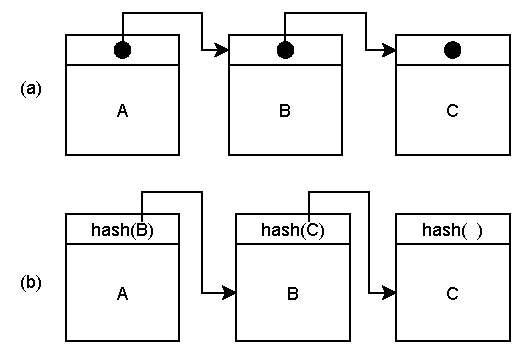
\includegraphics[width=.6\textwidth]{obrazky-figures/hash-pointer}
	\caption{(a) Zoznam pomocou ukazovateľov \medspace (b) Zoznam pomocou hash ukazovateľov}
	\label{img:hash-pointer}
\end{figure}

\subsection{Digitálny podpis}\label{subsec:sign}
Digitálny podpis (anglicky \textit{digital signature}) je kryptografický koncept používaný na autentifikáciu, autorizáciu a nepopierateľnosť. Digitálny podpis jednoznačne prepojí určitú entitu s informáciu. V technológii blockchain slúži digitálny podpis na určenie vlastníctva zdrojov, ktoré blockchain uchováva.~\cite{cryptoHandbook, satoshiBitcoin}

Moderná kryptografia používa pre zaistenie dôvernosti šifrovanie pomocou tajného kľúča. Pre zašifrovanie a dešifrovanie tajnej správy je potrebná znalosť tajného kľúča. Tento mechanizmus  zaisťuje dôvernosť avšak nezaisťuje nepopierateľnosť pretože obe komunikujúce strany poznajú tajný kľúč a teda nie je možné právne dokázať kto správu napísal. Na zaistenie nepopierateľnosti sa používa asymetrické šifrovanie, ktoré používa dvojicu kľúčov:
\begin{itemize}
	\item \textbf{Privátny kľúč} je tajný a pozná ho len odosielateľ správy. Odosielateľ používa tento kľúč na zašifrovanie správy.
	\item \textbf{Verejný kľúč} je dostupný komukoľvek. Ktokoľvek s týmto kľúčom dokáže dešifrovať správu.
\end{itemize}
Tieto dva kľúče tvoria dvojicu prepojenú matematickým spôsobom. Zo znalosti verejného kľúča je výpočetne nezvládnuteľné zistiť privátny kľúč. Zašifrovaná správa nie je dôverná pretože ktokoľvek môže použiť verejný kľúč na jej dešifrovanie. Avšak zašifrovaná správa je nepopierateľne napísaná vlastníkom privátneho kľúča. 

Tento koncept je základom digitálneho podpisu. Ak chceme nepopierateľne dokázať, že nejaký dátový obsah (napríklad pdf dokument) sme vytvorili mi, tak vypočítame jeho hash (viď sekcia~\ref{subsec:hash}) a zašifrujeme ho naším privátnym kľúčom. Zašifrovaný hash priložíme k dokumentu. Príjemca dokumentu si následne pomocou verejného kľúča dešifruje hash priložený k správe a porovná si ho s tým ktorý vypočítal sám z danej správy. Ak sú hashe rovnaké tak nikto správu nezmenil a dokument je jednoznačne vytvorený vlastníkom tajného kľúča. Najznámejšie algoritmy na digitálny podpis sú RSA, DSA, ECDSA.~\cite{cryptoHandbook}


\section{Peer-to-peer sieť}\label{sec:p2p}

Technológia blockchain je postavená na peer-to-peer sieťach. Peer-to-peer sieť sa podieľa na decentralizovanosti, nemennosti a auditovateľnosti blockchainu. 

Peer-to-peer sieť je dynamický súbor nezávislých uzlov (anglicky \textit{peers}), ktoré sú prepojené do grafu. Každý uzol obsahuje zdroje, ktoré zdieľa všetkým ostatným uzlom v sieti.~\cite{p2pBuford, p2pSchollmeier} Dôvod existencie peer-to-peer sietí je teda decentralizovaný spôsob zdieľania zdrojov ako sú súbory, fyzické zariadenia, výpočetný výkon alebo aj elektronické finančné zdroje. Dnes existuje množstvo peer-to-peer sietí. Veľmi známe sú napríklad Gnutella, Kazaa alebo BitTorrent.~\cite{p2pEssence}

\subsection{Referenčný model}
Najbežnejšie technické riešenie peer-to-peer siete je navrstvenie siete (anglicky \textit{overlay network}) na už existujúcu sieť, ktorou je typicky Internet. Takúto sieť potom môžeme definovať ako päticu $(P,R,I,F_P,F_R)$, kde:
\begin{itemize}
	\item $P$ je množina uzlov
	\item $R$ je množinu zdrojov
	\item $I$ je priestor identifikátorov
	\item $F_P: P \rightarrow I$ je funkcia, ktorá mapuje uzoly na identifikátory
	\item $F_R: R \rightarrow I$ je funkcia, ktorá mapuje zdroje na identifikátory
\end{itemize}

Obrázok~\ref{img:p2p-ref-model} ukazuje princíp fungovania takto definovanej siete. Tvorba siete s týmto modelom je potom závislá od šiestich návrhových aspektov:
\begin{enumerate}
	\item Voľba priestoru identifikátorov.
	\item Mapovanie zdrojov a uzlov na identifikátory.
	\item Správa priestoru identifikátorov v réžii uzlov siete.
	\item Tvorba grafu (štruktúra siete).
	\item Stratégia smerovania (anglicky \textit{routing}).
	\item Stratégia údržby.
\end{enumerate}
Konkrétne riešenie pre popisovaných šesť aspektov je zavislé od požiadaviek na efektivitu, škálovateľnosť, samoorganizovateľnosť, odolnosť voči chybám a kooperáciu.~\cite{p2pEssence}

\subsection{Využitie v blockchaine}

Peer-to-peer sieť umožňuje blockchainu uchovávať jeho obsah decentralizovane a pritom bezpečne. Tento koncept si vysvetlíme na prípade blockchainu, ktorý sa využíva ako kryptomena.

Elektronické financie sú typicky reprezentované pomocou elektronických mincí. Takáto minca je reprezentovaná pomocou nejakej sekvencie bitov. Avšak narozdiel od fyzických mincí, elektronické mince umožňujú jednoduchú falzifikáciu. Útočník skopíruje bitový reťazec danej mince a zaplatí ním viacnásobne rôzne produkty. Tento útok sa volá zdvojnásobenia výdavkov (anglicky \textit{double-spending attack}). Proti tomuto útoku existuje tradičné zabezpečenie pomocou centrálnej autority. Banka je centrálna autorita, ktorá schvaľuje všetky manipulácie s elektronickými mincami a teda neumožní použiť mincu takýmto podvodným spôsobom. Avšak toto riešenie nie je možné použiť v decentralizovanej sieti, kde centrálna autorita neexistuje. V prípade decentralizovanej siete je možné zabrániť tomuto útoku pomocou použitia dátovej štruktúry blockchain.~\cite{doubleSpending}

Kryptomena Bitcoin ako prvá navrhla použitie peer-to-peer siete v spojení s blockchain technológiou pre zabránenie double-spending útoku. V takejto sietu je jediný zdroj na zdieľanie a to je dátová štruktúra blockchain v ktorej sú uložené všetky informácie o elektronických financiách. Zjednodušene môžeme povedať, že majorita uzlov siete zdieľa rovnaký zdroj (rovnakú kópiu blockchainu). Ak chce niektorý uzol vykonať finančnú transakciu tak zašle správu s navrhovanou zmenou blockchainu do siete. Uzly v tejto sieti nie je potrebné identifikovať pretože správy posielané v tejto sieti nie sú smerované na žiadne konkrétne miesto. Keď uzol prijme správu s nejakou modifikáciu tak si overí či ide o validnú požiadavku na finančnú transakciu. Štruktúra blockchainu používa modernú kryptografiu na overenie validnosti transakcie (pozri sekciu~\ref{sec:crypto}). Blockchain, ktorý vlastní väčšina siete je ten, ktorý sa považuje za pravdu. Útočník by musel teda vlastniť aspoň 51\,\% uzolov v sieti aby mohol vykonať double-spending útok. Ak je daná sieť dostatočne veľká tak by toho útočník nemal byť schopný dosiahnuť.~\cite{satoshiBitcoin}

\begin{figure}[bt]
	\centering
	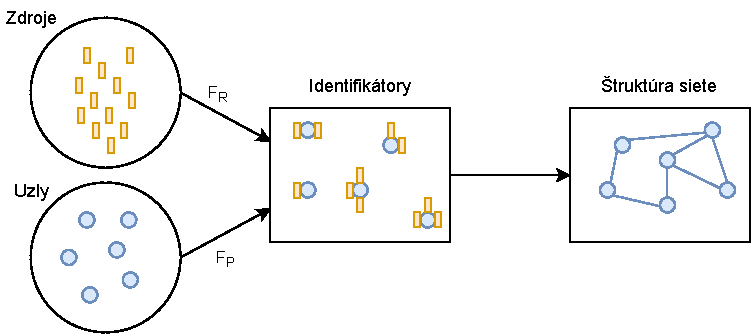
\includegraphics[width=\textwidth]{obrazky-figures/p2p-ref-model.pdf}
	\caption{Referenčný model peer-to-peer siete.~\cite{p2pEssence}}
	\label{img:p2p-ref-model}
\end{figure}

\section{Datová štruktúra blockchain}\label{sec:data-struct-blockchain}
Blockchain je dátová štruktúra podobná zoznamu (anglicky \textit{linked list}). Blockchain organizuje dáta do podmnožín, ktoré sa volajú bloky. Blok je podobný uzlu v zozname. Každý blok obsahuje referenciu na ďalší blok. Rozdiel medzi zoznamom a blockchainom je v tom, že referencia blockchainu je zabezpečená proti manipulácia (anglicky \textit{tamper-evident}) pomocou modernej kryptografie. Bežný zoznam používa referenciu pomocou ukazovateľov (anglicky \textit{pointers}), ktoré môže ktokoľvek a kedykoľvek pozmeniť bez toho aby pozmenil dátový obsah. Naopak, blockchain vôbec neumožňuje meniť už pridané bloky. Jediná povolená operácia je pridanie ďalšieho bloku na koniec blockchainu.~\cite{horizenAcademy}

Každý blok obsahuje dáta, ktoré sú typicky vo forme transakcií. Kryptograficky bezpečný blockchain by mohol fungovať aj tak, že v každom bloku bude uložená práve jedna transakcia. Z dôvodu optimalizácie je ale v jednom bloku uložené množstvo transakcií. Vďaka tejto optimalizácii nemusí celá sieť vytvárať konsenzus po každej transakcii. Samotné transakcie v rámci jedného bloku sú ukladané v ďalšej dátovej štruktúre, ktorá taktiež používa kryptografické hashovanie (viď sekcia~\ref{subsec:merkle-tree}).~\cite{narayanan2016bitcoin}

\subsection{Blok}\label{subsec:block}

Blok sa skladá z hlavičky a tela. Telo bloku obsahuje dáta a hlavička obsahuje metadáta. Dáta v tele bloku sú uložené vo forme transakcií. Transakcie sú popísané v sekcii~\ref{subsec:transaction}. Počet transakcií v bloku je typicky obmedzený maximálnou veľkosťou bloku.
Hlavička bloku obsahuje metadáta o bloku, kde najdôležitejšie a najbežnejšie sú nasledujúce:
\begin{itemize}
	\item Hash všetkých transakcií.
	\item Časové razítko vytvorenia bloku.
	\item Hash ukazovateľ na predošlý blok v blockchaine.
	\item Náhodná výzva (anglicky \textit{nonce}), ktorej využitie vysvetľuje sekcia~\ref{subsec:pow}
\end{itemize} 

~\cite{zhengBlockchainOverview}


\subsection{Transakcia}\label{subsec:transaction}
Transakcia je elementárna dátová jednotka na ukladanie dáta v blockchaine. Bitcoin, prvý blockchain, použil transakciu na manipuláciu s elektronickými financiami. Takáto transakcia sa skladá z troch častí:
\begin{itemize}
	\item \textbf{Množina vstupov}: Každý vstup má uložený hash predošlej transakcie s ktorej vychádza. Ďalej definuje, ktoré výstupy s predošlej transakcie si nárokuje. Nakoniec obsahuje digitálny podpis, ktorý autorizuje tvorcu transakcie.
	\item \textbf{Množina výstupov}: Každý výstup má hodnotu, ktorá je uchovávaná v blockchaine (typicky minca nejakej kryptomeny). Suma hodnôt všetkých výstup transakcie musí byť menšia alebo rovná sume všetkých vstupov transakcie. Ak je menšia, tak tento rozdiel je použitý ako odmena pre toho, kto publikoval tento blok blockchainu.
	\item \textbf{Hlavička}: Obsahuje hash transakcie, ktorý je používaný ako unikátny identifikátor pomocou, ktorého sa na transakciu odkazujeme.
\end{itemize}


\subsection{Binárny hashovací strom}~\label{subsec:merkle-tree}
Binárny hashovací strom alebo tiež Merkle strom (anglicky \textit{Merkle tree}) je datová štruktúra podobná binárnemu stromu, ktorá slúži na efektívne a rýchle vypočítanie hashu veľkého množstva dát. Blockchain používa tento strom na časovo efektívny výpočet hashu všetkých transakcií. Takto vypočítaný hash je uložený v hlavičke bloku.

Merkle strom je vyvážený binarny strom, kde listové uzly obsahujú jednotlivé transakcie uložené v danom bloku blockchainu. Každý nelistový uzol stromu obsahuje hash vypočítaný z jeho potomkov. Koreňový uzol teda obsahuje hash celého stromu a teda aj všetkých transakcií. Pridanie, odobranie, zmena obsahu, alebo zmena poradia transakcií bude teda viesť k zmene koreňového hashu. Konštrukcia stromu, inak povedané výpočet hashu všetkých transakcií, prebieha následovne:
\begin{enumerate}
	\item Všetky transakcie sú uložené do listovej úrovne stromu. Ak je počet transakcií nepárny tak, je posledná vložená dvakrát.
	\item Nad každým listovým uzlom je vypočítaný hash.
	\item Každý nelistový uzol skonkatenuje hash ľavého a pravého syna, vypočíta nad nimi hash a uloží si ho. 
\end{enumerate}
Konštrukcia takéhoto stromu pre $n$ transakcií má časovú zložitosť $O(log(n))$. Takýto spôsob výpočtu hashu je teda veľmi efektívny pre veľké množstvo transakcií (blok v blockchaine bežne obsahuje stovky transakcií).~\cite{merkleTreeBosamia}

Merkle strom umožnuje efektívne šetriť pamäťové nároky blockchainu. Do blockchainu sú neustále pridávané nové bloky, ktoré obsahujú aj rovnaké staré transakcie. Ak už sú transakcie zaznamenané v dostatočne veľkom množstve blokov tak sú z hľadiska bezpečnosti nemenné. V nových blokoch ich už preto nie je potrebné ukladať. Nový blok si preto uloží len hashe starých vetiev stromu, ale ich obsah už nepotrebuje. Takto je zachovaná integrita hashu všetkých transakcií.~\cite{satoshiBitcoin}

\section{Ťažba blokov}\label{sec:mining}

Ťažba (anglicky \textit{mining}) bloku je proces pridania nové bloku na koniec blockchainu. Ťažba bloku zahŕňa validáciu transakcií a blokov. Preto je ťažba kritická pre správne a bezpečné fungovanie blockchainu. Každý uzol siete, ktorý ťaží nové bloky sa nazýva anglickým slovom \textit{miner}. Tieto uzly umožňujú rozširovanie blockchainu. Aby takéto uzly existovali, musia byť motivované. Miner dostane za každý vyťažený blok ako odmenu zdroje uložené v blockchaine.

Ťažba všeobecne pozostáva z nasledujúcich krokov:
\begin{enumerate}
	\item Miner prijíma požiadavky na transakcie z peer-to-peer siete. Každú transakciu si validuje pomocou kryptografie popísanej v sekcii~\ref{sec:crypto}.
	\item Miner musí taktiež udržiavať aktuálny stav blockchainu. Je potrebné sledovať či nevznikli nové bloky a udržiavať si validný blockchain.
	\item Ak miner vlastní validnú a aktuálnu kópiu blockchainu, môže začať vytvárať nový blok. Do nového bloku vloží transakcie, ktoré prijal a boli validné.
	\item Novo vytvorený blok je potrebné distribuovať do siete. Ak väčšina siete blok získa a akceptuje, tak bol pridaný do blockchainu. Tento proces zahŕňa problém konsenzu v sieti, ktorý je podrobne vysvetlený v sekcii~\ref{sec:consenzus}.
	\item Ak sa podarilo úspešne blok pridať do blockchainu tak miner získava odmenu. Odmena za vyťažený blok je konštantná čiastka zdrojov poskytovaných daným blockchainom. Napríklad Bitcon poskytuje v roku 2021 ako odmenu 6,25 bitcoinov čo približne 300 dolárov~\footnote{\url{https://www.investopedia.com/tech/how-does-bitcoin-mining-work/}}. Avšak táto odmena môže byť navýšená o poplatky, ktoré sú v transakciách. Ak teda chcete aby sa vaša transakcia dostala do blockchainu čo najrýchlejšie, poskytnete vyššiu odmenu v podobe poplatku za transakciu. Miner bude potom viac motivovaný pridať práve túto transakciu do bloku.
\end{enumerate}

~\cite{narayanan2016bitcoin}

\section{Konsenzus}\label{sec:consenzus}
Konsenzus v blockchaine zabezpečuje, že skupina uzlov (peerov) sa  zhodne na rovnakom stave blockchainu. Tradične je konsenzus zabezpečený centrálnou autoritou s ktorou musia byť všetky uzly spojené. Avšak blockchain je decentralizovaný a teda toto riešenie nie je možné. Konsenzus v decentralizovanej sieti blockchainu je zabezpečený pomocou protokolu, ktorý sa snaží nájsť kompromis medzi nasledujúcimi vlastnosťami~\cite{gilbertCAP, zhangConsensus, leporeConsensus}:
\begin{itemize}
	\item Konzistentnosť: Vždy keď dôjde k potvrdeniu zmeny, celý reťazec sa aktualizuje a všetci čítajú rovnaké hodnoty.
	\item Dostupnosť: Pre každú požiadavku na dáta musí byť poskytnutá odpoveď.
	\item Odolnosť voči prerušeniu (anglicky \textit{partial tolerance}): Sieť funguje aj v prípade, že v nej vznikajú chyby.
\end{itemize}

Existujú tri najbežnejšie techniky, ktoré sa používajú pre ustavenie konsenzu~\cite{homoliakBlockchain}:
\begin{itemize}
	\item \textbf{Lotéria}: Takéto protokoly náhodne zvolia uzol, ktorý vyprodukuje nový blok. Výhodou tohoto prístupu je jeho jednoduchosť keďže takýto proces nevyžaduje žiadnu interaktivitu. Nevýhodou tohoto prístupu je, že pripúšťa možnosť voľby viacerých uzlov súčasne. V takom prípade sa reťazec rozvetví (anglicky \textit{fork}) a je potrebné určiť ktorá vetva je správna. Typicky sa za správnu vetvu volí tá najdlhšia. Avšak takéto správanie oslabuje konzistentnosť blockchainu. Transakcie v posledných blokoch môžu byť potenciálne zahodené pretože nejde o správnu vetvu. Preto sa za konzistentné transakcie považujú až tie ktoré sú prekryté väčším množstvom nových blokov.
	\item \textbf{Hlasovanie}: Protokoly založené na hlasovaní dosahujú dohodu pomocou hlasovania všetkých zapojených uzlov. Môžeme použiť napríklad protokol Byzantskej chyby (anglicky \textit{Byzant fault tolerance}), ktorý vyžaduje majoritu hlasov k uzavretiu konsenzu (typicky $\frac{2}{3}$). Výhodou je veľmi malá pravdepodobnosť vzniku vetiev reťazca. Na druhej strane, takéto protokoly majú nižšiu priepustnosť, ktorá klesá z narastajúcim počtom uzlov.
	\item \textbf{Kombinovaný prístup}: Tieto protokoly sa snažia kombinovať prístup lotérie a hlasovania s cieľom dosiahnuť výhody oboch prístupov. Napríklad je možné rozdeliť počet uzlov podieľajúcich sa na hlasovaní pomocou lotérie, čím sa zvýši priepustnosť.
\end{itemize}
~\cite{zhangConsensus, homoliakBlockchain}

\subsection{Proof-of-Work}\label{subsec:pow}
Dôkaz prácou (anglicky \textit{proof of work}) je najbežnejšia stratégia konsenzus protokolu. Ak chce uzol publikovať nový blok, musí investovať svoj výpočtový výkon do riešenia netriviálneho kryptografického problému. Uzol, ktorý ako prvý vyrieši tento problém má najväčšiu pravdepodobnosť, že bude jeho blok pridaný do reťazca. Samozrejme, je tu možnosť, že problém vyrieši súčasne viacero uzlov. Konečná voľba je teda náhodná. Proof-of-work teda umožňuje, aj keď s oveľa menšou pravdepodobnosťou, že sa reťazec rozvetví. Bezpečnosť takéhoto konsenzu spočíva v tom, že majorita výpočtového výkonu siete (51\,\%) je vlastnená poctivými uzlami.~\cite{leporeConsensus}

Samotný kryptografický problém, ktorý sa rieši spočíva v počítaní hashu (viď~\ref{subsec:hash}) z hlavičky nového bloku (viď~\ref{subsec:block}). Hlavička obsahuje atribút nonce, ktorý môže miner ľubovolne nastaviť. Zmenou tohoto atribútu môže miner získať iný hash hlavičky bloku. Konsenzus vyžaduje aby výsledná hash hodnota bola menšia rovná určitej zvolenej hodnote. Miner môže túto podmienku dosiahnuť len tak, že bude inkrementovať hodnotu atribútu nonce až dokedy túto podmienku nesplní. Táto úloha sa teda dá riešiť len pomocou metódy útok hrubou silou (anglicky \textit{brute force}). Miner môže svoju šancu na úspech zvýšiť len tým, že poskytne väčší výpočtový výkon do jej riešenia. Na druhej strane, ostatné uzly môžu overiť, že jeho riešenia je správne veľmi rýchlo a efektívne.~\cite{zhengBlockchainOverview}

Proof-of-work konsenzus využíva dva typy uzlov. Prvý typ uzla je miner, ktorý vytvára nové bloky tak ako je popísané v sekcii~\ref{sec:mining}. Druhý typ uzla je bežný vlastník zdrojov v danom blockchaine, ktorý môže vytvárať transakcie a distribuovať ich do siete. Druhý typ uzla teda nehrá žiadnu rolu v ustanovovaní konsenzu.~\cite{leporeConsensus}

Proof-of-work je overený konsenzus protokol, ktorý funguje a používa sa v blockchainoch ako je Bitcoin~\cite{satoshiBitcoin} alebo Ethereum~\footnote{\url{https://ethereum.org/en/whitepaper/}}. Tento protokol má však jeden dlhodobý problém a to je spotreba energie. Uzly ktoré riešia kryptografický problém pre nové bloky spotrebujú veľké množstvo energie čo má nepriaznivý dopad na životné prostredie. Niektoré zdroje~\footnote{\url{https://www.businessinsider.com/bitcoin-mining-electricity-usage-more-than-google-2021-9}} napríklad hovoria, že v roku 2021 pokrýva ťažba Bitcoinu 0,5\,\% celkovej spotreby elektrickej energie na svete. Pre porovnanie, ide o sedemkrát väčšiu spotrebu energie ako má celá spoločnosť Google.~\cite{leporeConsensus}

\subsection{Proof-of-Stake}\label{subsec:pos}


%===============================================================================
